%--------Preliminares
%--------Emir Muñoz Jiménez
%--------13-10-2010

\chapter{Marco Te\'orico}
\label{cap:preliminares}

\section{Impresión 3D}

 A diferencia de las técnicas principales que se emplean desde hace algunos años en la fabricación de objetos, que se encargan de sustraer, combinar, o deformar paulatina y controladamente materia hasta llegar a una pieza final, la impresión 3D funciona de un modo completamente distinto. La pieza se crea en un solo paso, capa por capa, a un ritmo medio de uno a dos centímetro de altura por hora; el objeto creado puede constar de mecanismos internos (como rodamientos de bolas), formas tejidas y entrelazadas, o incluso huecos y curvas \citep{Berchon2014}. Pues bien, todas las impresoras 3D, están basadas sobre el mismo principio: un modelo digital es transformado a un objeto físico de 3 dimensiones por adición de material en capas. Esto se conoce alternativamente como \textit{Manufactura Aditiva} \citep{3dhub2018}. Este tipo de fabricación también se puede englobar dentro de lo que se denomina \textit{Fabricación digital}, cuyo principio básico es la transformación de la información  desde el mundo físico al digital. Según \citep{jorquera2016}, la fabricación digital incluye los siguientes sistemas y tecnologías:
 
 \begin{itemize}
	
	\item[Sistemas integrados:] Es un \textit{hardware} electrónico diseñado específicamente para llevar a cabo una o pocas tareas definidas. Las impresoras llevan un sistema electrónico integrado que utilizan para controlar los motores paso a paso que alimentan el papel, recibir información de los sensores de temperatura y finales de carrera, o que mandan al cabezal de impresión.
	\item[Sistemas CNC (\textit{Computer Numeric Control} - control numérico computarizado):] Es el control numérico de un sistema de automatización que se utiliza para controlar diferentes máquinas herramienta. Este sistema ha revolucionado la industria gracias a la simplificación del \textit{software} de diseño en conjunto con los lenguajes de programación como el \textit{.gcode}. Esencialmente, un sistema CNC es cualquier sistema que utiliza un ordenador para controlar los movimientos de una máquina.
	\item[Software CAD (\textit{Computer Aided Design}- diseño asistido por computador):] es, en esencia, un programa que sirve para la creación, edición análisis y visualización de modelos tridimensionales.  
	
 
 \end{itemize}

\subsection{Historia de la impresión 3D}

\subsection{Métodos de impresión 3D}

\subsection{Impresoras 3D FDM}

\subsection{Tipologías de impresión 3D FDM}

\section{Mantenimiento}

\subsection{Historia y evolución del mantenimiento}

\subsection{Tipos de mantenimiento}

\subsection{GMAO}

\section{Lean Manufacturing}

\subsection{Historia Lean Manufacturing}

\subsection{Herramientas de mantenimiento}

\section{Design Thinking y Scrum}

\subsection{Metodologías ágiles}

\subsection{Scrum}

\subsection{Design Thinking}

\subsection{Fases del Design Thinking}

\subsection{Herramientas para diseño de Software}

\section{Desarrollo de Software}

\subsection{Programación orientada a objetos}

\subsection{Lenguajes de programación}

\subsection{Arquitectura Cliente-Servidor}

\subsection{API}

\subsection{Ordenadores de placa reducida}

 \ldots 

 

% Figura: \'Arbol XML 1
%\begin{figure}[tp]
%  \centering
%  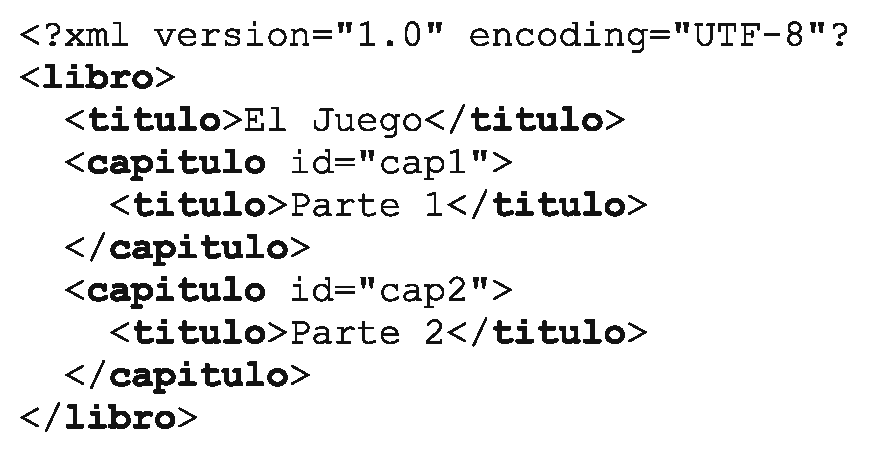
\includegraphics[scale=.5]{images/XML-document-example1}
%  \caption{\em Modelo de árbol para un documento XML.}
%  \label{fig:xml-tree-exa1}
%\end{figure}



